\documentclass{article}

\usepackage{graphicx}
\usepackage{tikz}
\usepackage{tikzsymbols}
\usetikzlibrary{calc,patterns,shapes.geometric}
\pagestyle{empty}
\usepackage[margin=0pt]{geometry}
\geometry{papersize={14in,12in}}

\def\centerarc[#1](#2)(#3:#4:#5){\draw[#1] ($(#2)+({#5*cos(#3)},{#5*sin(#3)})$) arc (#3:#4:#5);}

\begin{document}
	\begin{figure}
		\centering
		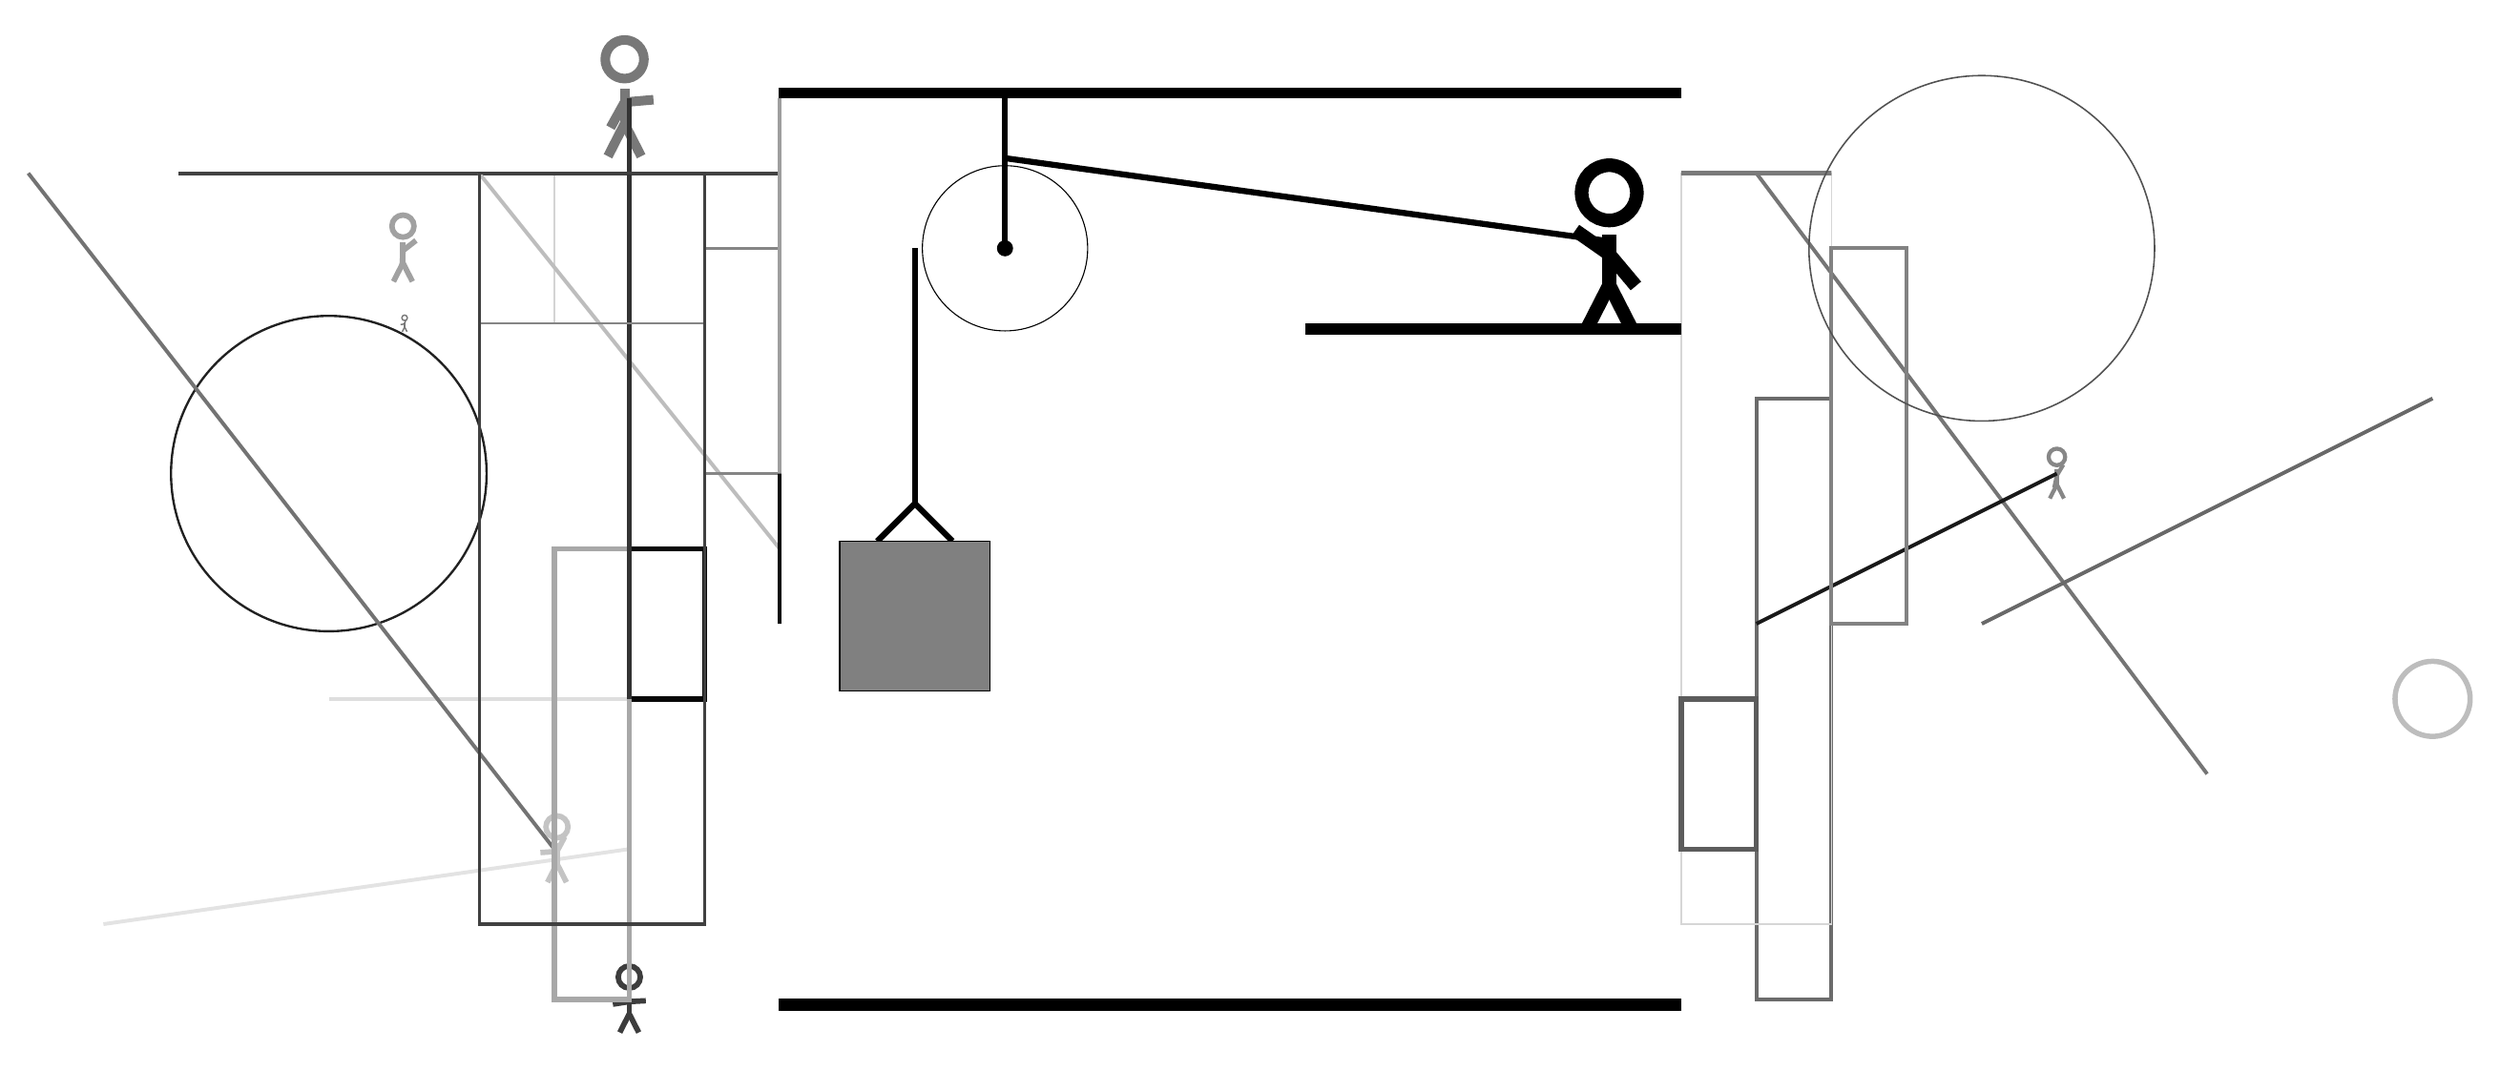
\begin{tikzpicture}
			%%%%% START %%%%%
			
			\draw[fill=black] (-2, 9) rectangle (10, 9.125);
			
			\draw[line width=0.2mm, color=black!17] (-3, 6) rectangle (-5, 8);
			
			\node[line width=0.6mm, color=black!47] at (15, 4) {\Strichmaxerl[3][78][59]};
			\draw[line width=0.5mm, color=black!11](-4, -1) -- (-11, -2);
			\node[line width=0.6mm, color=black!76] at (-4, -3) {\Strichmaxerl[4][9][3]};
			
			\draw [line width=0.3mm, color=black!87](-8, 4) circle (2.1);
			
			\draw[line width=0.5mm, color=black!13](-3, 1) -- (-8, 1);
			\node[line width=0.5mm, color=black!37] at (-7, 7) {\Strichmaxerl[4][87][38]};
			
			\draw[line width=0.5mm, color=black!55](-5, -1) -- (-12, 8);
			\draw[line width=0.7mm, color=black!97] (-4, 3) rectangle (-3, 1);
			\node[line width=0.2mm, color=black!23] at (-5, -1) {\Strichmaxerl[4][4][62]};
			
			\draw[line width=0.5mm, color=black!58] (11, 5) rectangle (12, -3);
			
			\draw[line width=0.5mm, color=black!74](-2, 8) -- (-10, 8);
			\draw[line width=0.7mm, color=black!34] (-4, 3) rectangle (-5, -3);
			
			\node[line width=0.6mm, color=black!53] at (-4, 9) {\Strichmaxerl[7][61][5]};
			\node[line width=0.2mm, color=black!53] at (-7, 6) {\Strichmaxerl[1][8][74]};
			\draw[line width=0.5mm, color=black!26](-2, 3) -- (-6, 8);
			
			\draw[line width=0.5mm, color=black!54](11, 8) -- (17, 0);
			\draw[line width=0.4mm, color=black!48] (-2, 7) rectangle (-3, 4);
			\draw[line width=0.5mm, color=black!59](14, 2) -- (20, 5);
			\draw[line width=0.2mm, color=black!16] (10, -2) rectangle (12, 8);
			\draw[line width=0.6mm, color=black!52] (10, 8) rectangle (12, 8);
			
			\draw[line width=0.5mm, color=black!90](11, 2) -- (15, 4);
			
			\draw[line width=0.5mm, color=black!49] (12, 7) rectangle (13, 2);
			\draw[line width=0.7mm, color=black!80] (-4, 1) rectangle (-4, 9);
			\draw [line width=0.7mm, color=black!26](20, 1) circle (0.5);
			
			\draw[line width=0.2mm, color=black!48] (-3, 6) rectangle (-6, 6);
			\draw[line width=0.4mm, color=black!75] (-3, 8) rectangle (-6, -2);
			\draw[line width=0.5mm, color=black!97] (-2, 6) rectangle (-2, 2);
			\draw [line width=0.2mm, color=black!68](14, 7) circle (2.3);
			
			\draw[line width=0.7mm, color=black!64] (11, -1) rectangle (10, 1);
			\draw[line width=0.6mm, color=black!38] (-2, 9) rectangle (-2, 4);
			
			\draw (1, 7) circle (1.1);
			\draw[fill=black] (1, 7) circle (0.1);
			\draw[line width=0.8mm] (1, 9) -- (1, 7);
			
			\draw[line width=0.8mm](-0.7, 3.1) --  (-0.2, 3.6) -- (0.3, 3.1);
			\draw[fill=black!50] (-1.2, 3.1) rectangle (0.8, 1.1);
			
			\draw[line width=0.8mm](-0.2, 7) -- (-0.2, 3.6);
			\centerarc[line width=0.8mm](1, 7)(90:180:1.2000000000000002)
			\draw[line width=0.8mm](1, 8.2) -- (9, 7.1);
			
			\node at (9, 7) {\Strichmaxerl[10][-35][-50]};
			\draw[fill=black] (5, 6) rectangle (10, 5.85);
			
			\draw[fill=black] (-2, -3) rectangle (10, -3.15);
			
			%%%%% END %%%%%
		\end{tikzpicture}
	\end{figure}	
\end{document}